% Created 2018-11-13 Di 15:52
% Intended LaTeX compiler: pdflatex
\documentclass[11pt]{article}
\usepackage[utf8]{inputenc}
\usepackage[T1]{fontenc}
\usepackage{graphicx}
\usepackage{grffile}
\usepackage{longtable}
\usepackage{wrapfig}
\usepackage{rotating}
\usepackage[normalem]{ulem}
\usepackage{amsmath}
\usepackage{textcomp}
\usepackage{amssymb}
\usepackage{capt-of}
\usepackage{hyperref}
\usepackage{minted}
\usepackage{float}
\author{Nikolai Weidt}
\date{\today}
\title{Calcback}
\hypersetup{
 pdfauthor={Nikolai Weidt},
 pdftitle={Calcback},
 pdfkeywords={},
 pdfsubject={},
 pdfcreator={Emacs 26.1 (Org mode 9.1.14)}, 
 pdflang={English}}
\begin{document}

\maketitle
\setcounter{tocdepth}{2}
\tableofcontents



\section{What is this?}
\label{sec:org068f0f7}
This is a script to get the complex refractive index \(n = n * ik\) from the ellipsometric parameters \(\Delta\) and \(\Psi\) I got from a simulation.
The result for 300nm SiO\(_{\text{2}}\) should look like this:

\begin{figure}[htbp]
\centering
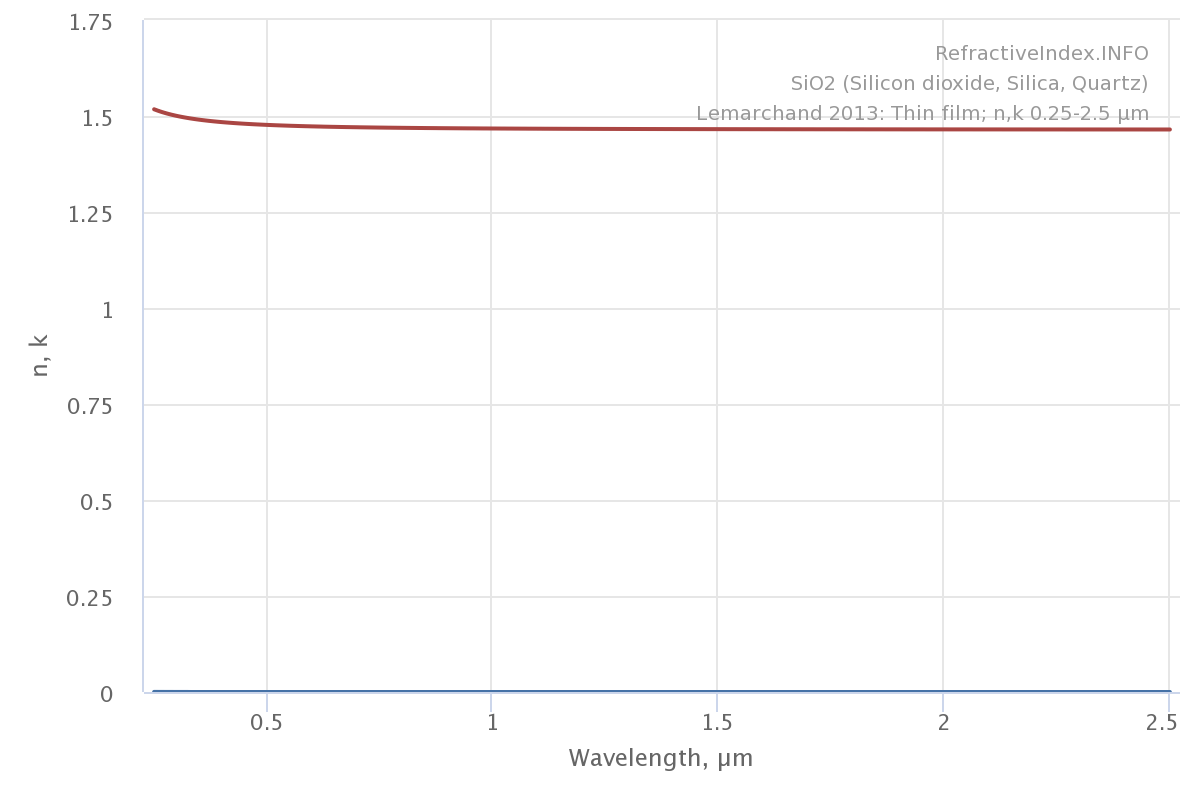
\includegraphics[width=\textwidth]{./RefractiveIndexSiO2.png}
\caption{\label{fig:org8ef2f84}
Refractive index should look like this}
\end{figure}
\section{List of Todos:}
\label{sec:orgeacd8a7}

\subsection{{\bfseries\sffamily TODO} Write a loop for all wavelengths after it works for one.}
\label{sec:org3ef5c64}
\subsection{{\bfseries\sffamily TODO} Then take even more wavelengths (rows)}
\label{sec:org891a926}
\section{Imports:}
\label{sec:org42b68b1}
\begin{minted}[]{python}
import numpy as np
import matplotlib
matplotlib.use('Agg')
import matplotlib.pyplot as plt
\end{minted}

\section{Defining some variables:}
\label{sec:org8bbb179}
Defining some variables for later use:

\begin{minted}[]{python}
CSVFILE = "100nmSiO2.csv"  # head300nmSiO2.csv = only 10 rows of data
phi_i = 70 * np.pi / 180  # converting incident angle from deg (first number) to rad
d_L = 100  # thickness of layer in nm
n_air = 1  # refractive index of air
rerange = 5  # upper limit for real part
imrange = 1  # upper limit for imaginary part
# i = 88  # only look at one wavelength (row in csv)
\end{minted}

\section{Read .csv-file:}
\label{sec:org95190ec}
Read the values into a two dimensional numpy array as [[lambda,Psi,Delta,n\(_{\text{S}}\), k\(_{\text{S}}\)],\ldots{}] (Skip columns 3 and 4)

\begin{minted}[]{python}
csv = np.loadtxt(CSVFILE, delimiter=",", skiprows=1)
\end{minted}

:DEBUG:
The array looks like this:
\begin{minted}[]{python}
csv
\end{minted}

\begin{verbatim}
[[ 4.00000000e+02  4.63752956e+01 -8.41522003e+01  5.62650000e+00
   3.30100000e-01]
 [ 4.01000000e+02  4.66645899e+01 -8.40149297e+01  5.59460000e+00
   3.18200000e-01]
 [ 4.02000000e+02  4.69702190e+01 -8.38513987e+01  5.56370000e+00
   3.07000000e-01]
 ...
 [ 7.98000000e+02  3.32352187e+01  1.00231229e+02  3.69890000e+00
   4.10000000e-03]
 [ 7.99000000e+02  3.31871064e+01  1.00206655e+02  3.69810000e+00
   4.00000000e-03]
 [ 8.00000000e+02  3.31422918e+01  1.00188647e+02  3.69740000e+00
   4.00000000e-03]]
\end{verbatim}

\section{Calculate \(\rho\)}
\label{sec:orgb3450dc}
\subsection{Create a matrix containing every possible refractive index (n+ik):}
\label{sec:org9c3a06d}

Change the last number in the "linspaces" to adjust the resolution.

\begin{minted}[]{python}
lsp_re = np.linspace(1, rerange, 1001)
lsp_im = np.linspace(0.01, imrange, 1001)
# re, im = np.meshgrid (lsp_re, lsp_im, copy=False)
# n_L = 1j * np.round(im,6) + np.round(re,6)
# n_L = n_L.flatten() # create onedimensional array
n_L = lsp_re
\end{minted}

This gives the following matrix:
\begin{minted}[]{python}
n_L
\end{minted}

\begin{verbatim}
[1.    1.004 1.008 ... 4.992 4.996 5.   ]
\end{verbatim}

\subsection{Calculate \(\rho\):}
\label{sec:org6938a55}
\subsubsection{First we define some functions:}
\label{sec:org990b6e3}
\begin{enumerate}
\item Snell's Law to calculate the refractive angles:
\label{sec:org03219ee}
Phi is the incident angle for the layer, n1 and n2 are refractive indices of first and second medium. Returns the angle of refraction.

\begin{figure}[H]
\centering
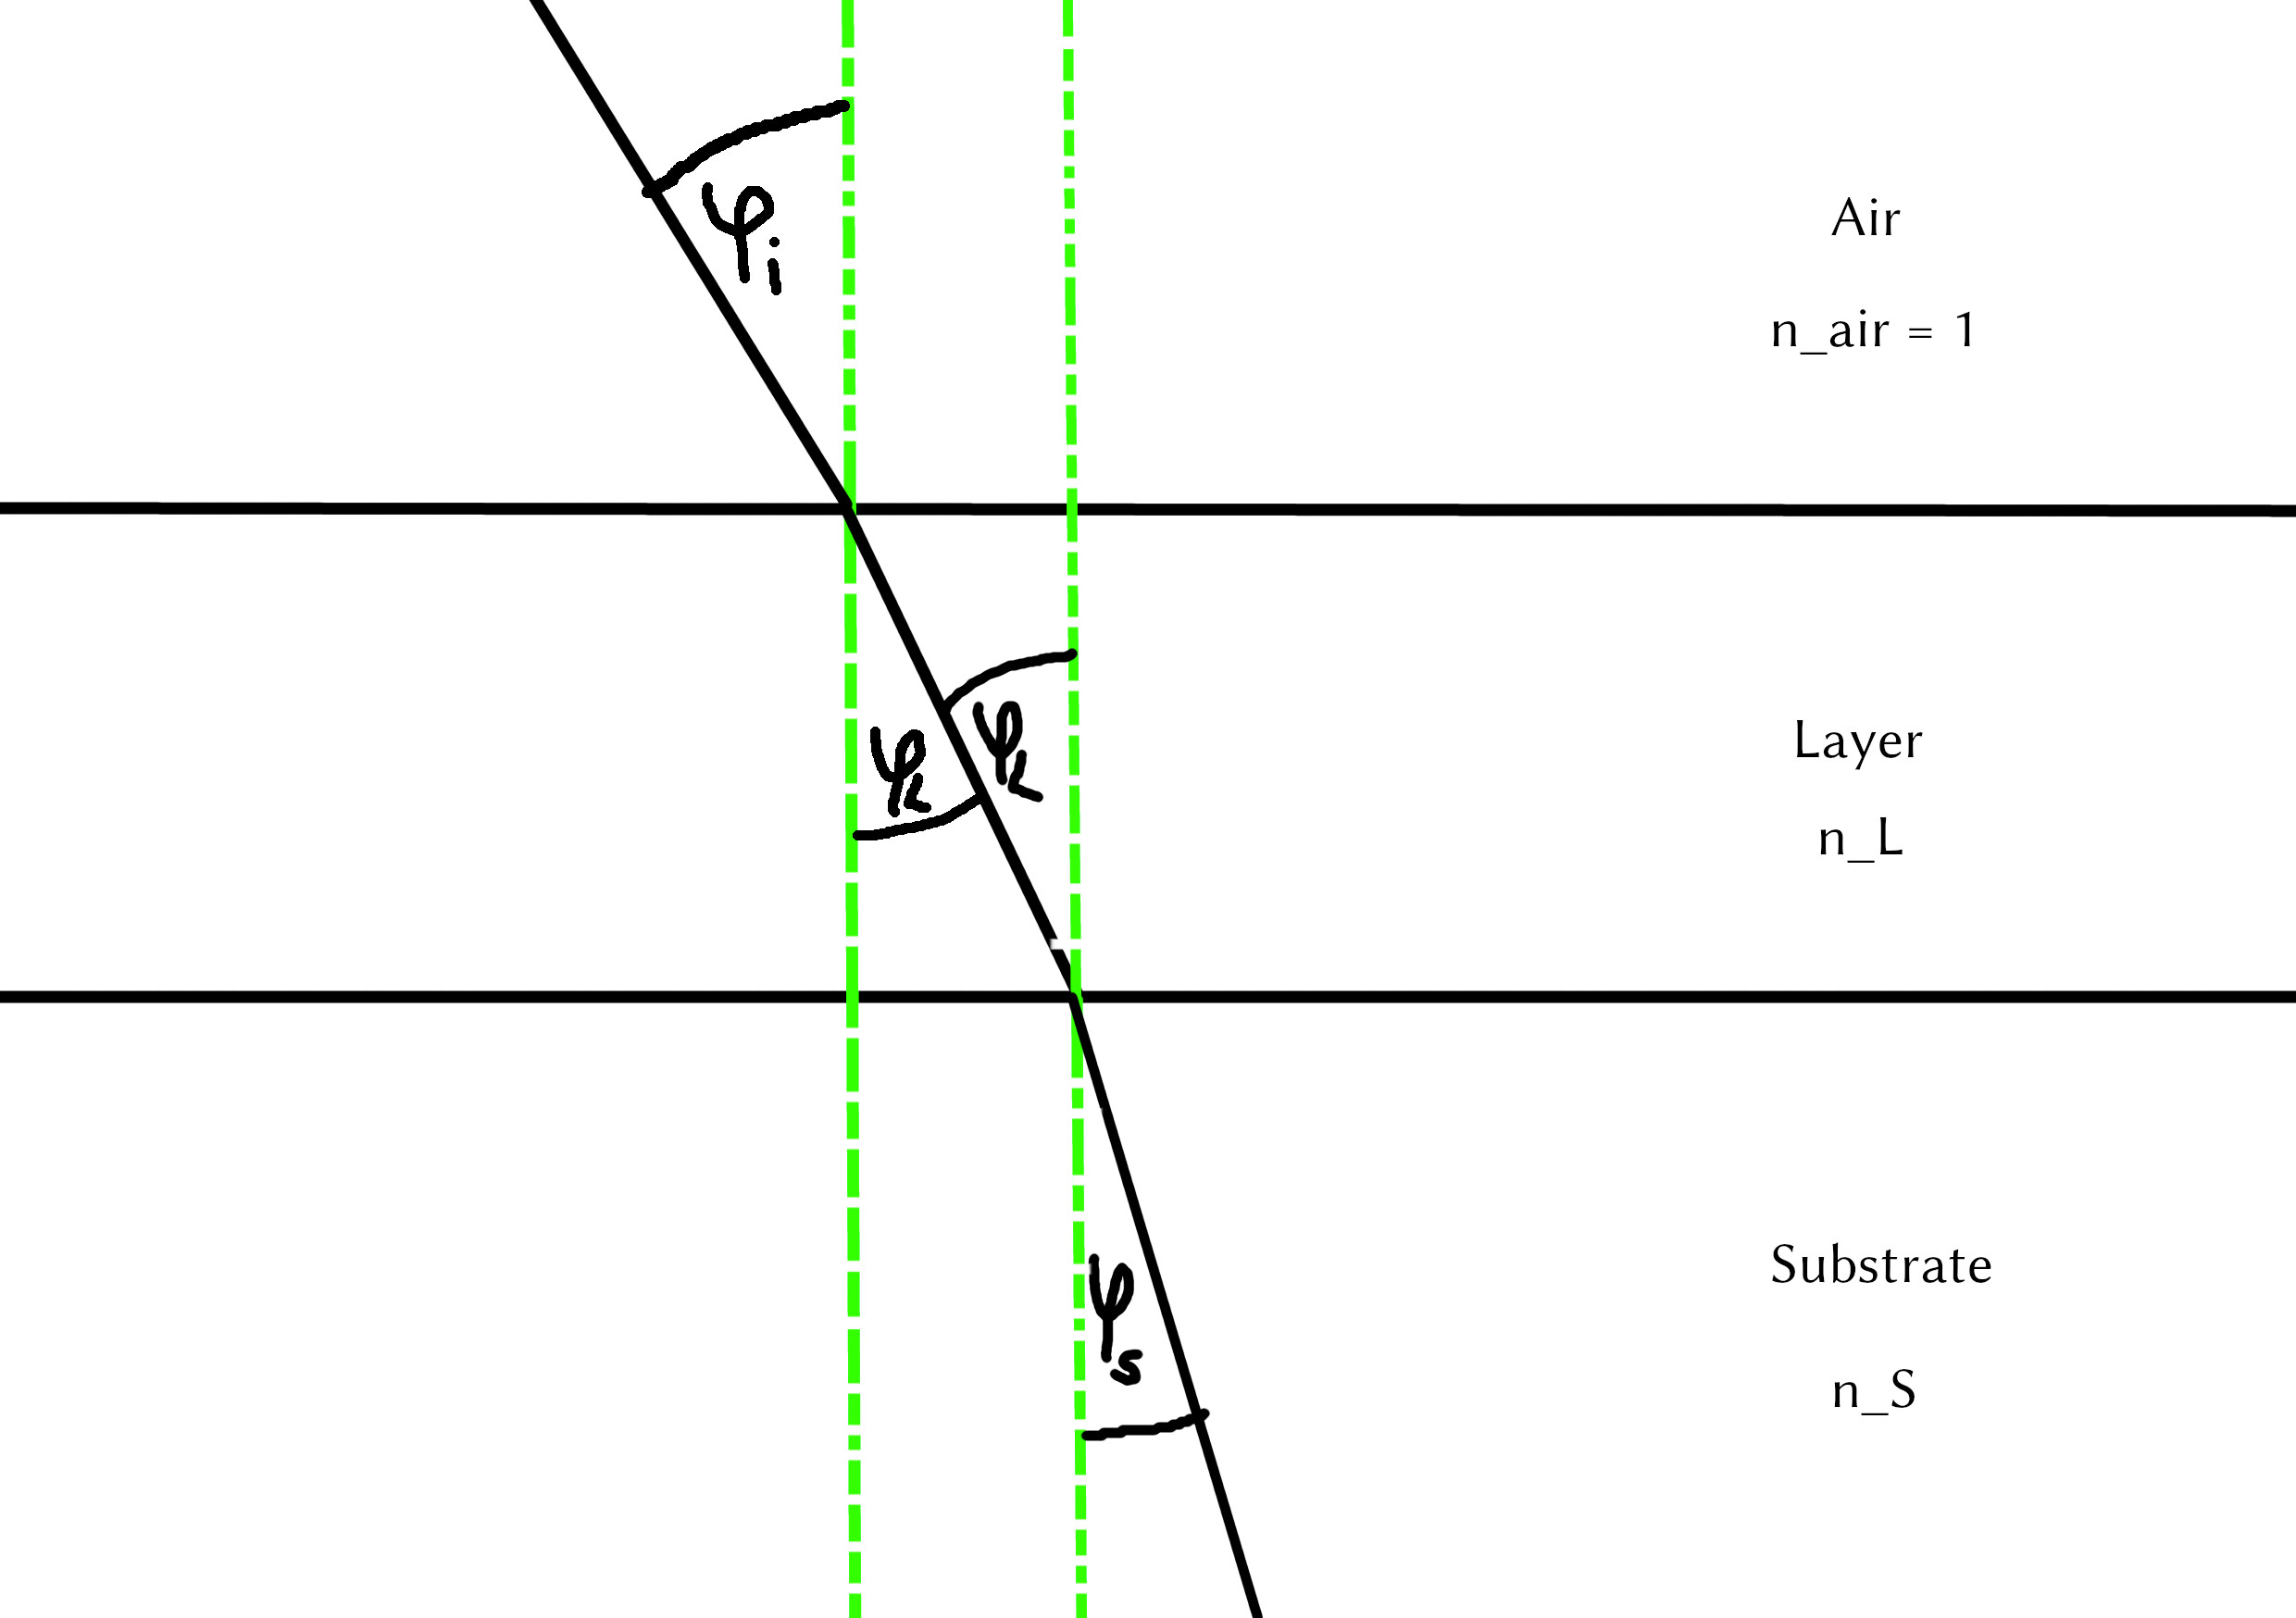
\includegraphics[width=\textwidth]{./snell.jpg}
\caption{\label{fig:orgcdb8128}
Snell's Law}
\end{figure}
\begin{minted}[]{python}
def snell(phi, n1, n2):
  """Calculates the refractive angle, parameters are incident angle phi, refractive index of first medium n1 and of second medium n2"""
  phi_ref = np.arcsin((n1/n2)*np.sin(phi))
  return phi_ref
\end{minted}


\item Calculate r\(_{\text{p}}\) and r\(_{\text{s}}\) with Fresnel equations:
\label{sec:orgd09a528}
\begin{minted}[]{python}
def fresnel(n1, phi1, n2, phi2):
    """Takes refractive indices and angles of two layers to calculate the amplitude reflection coefficients"""
    rs = (n1 * np.cos(phi1) - n2 * np.cos(phi2)) / (n1 * np.cos(phi1) + n2 * np.cos(phi2))
    rp = (n2 * np.cos(phi1) - n1 * np.cos(phi2)) / (n2 * np.cos(phi1) + n1 * np.cos(phi2))
    return rs, rp
\end{minted}


\item Calculate \(\rho\) for the layer with eq. 5.2 in Spectroscopic Ellipsometry \citenum{fujiwara2009spectroscopic}:
\label{sec:org50aedcb}
\begin{minted}[]{python}
def calc_diff(n_L, rho_giv):
    #Snell's Law:
    phi_L = snell(phi_i, n_air, n_L)
    phi_S = snell(phi_L, n_L, n_S)
    # Fresnel equations:
    # air/layer:
    rs_al, rp_al = fresnel(n_air, phi_i, n_L, phi_L)
    # layer/substrate:
    rs_ls, rp_ls = fresnel(n_L, phi_L, n_S, phi_S)

    beta = (2 * np.pi / lambda_vac) * d_L * n_L * np.cos(phi_L)
    rp_L = (rp_al + rp_ls * np.exp(-2 * 1j * beta)) / (
        1 + rp_al * rp_ls * np.exp(-2 * 1j * beta))
    rs_L = (rs_al + rs_ls * np.exp(-2 * 1j * beta)) / (
        1 + rs_al * rs_ls * np.exp(-2 * 1j * beta))
    rho_L = rp_L / rs_L
    return abs(rho_giv - rho_L), rho_L
\end{minted}
\end{enumerate}


\subsubsection{Then we call these functions one after another to calculate \(\rho\):}
\label{sec:orgf340923}
Get refractive index of the substrate (n\(_{\text{S}}\)) and lambda from the csv:
\begin{minted}[]{python}
lambda_vac = csv[i][0]
n_S = (csv[i][3] + 1j * csv[i][4])
\end{minted}


\subsubsection{Identify the best fitting rho with \(\rho\) = tan(\(\psi\)) * e\(^{\text{i}\Delta}\) :}
\label{sec:orgc6ab954}

\begin{minted}[]{python}
# psi is in our csv-file at index 1, delta at index 2 at row "i" for lambda
n_array = [] 
rho_array = []
for i, row in enumerate(csv):
    lambda_vac = csv[i][0]
    psi = csv[i][1] * (np.pi/180)
    delta = csv[i][2] * (np.pi/180)
    n_S = csv[i][3] + csv[i][4] * 1j
    rho_giv = np.tan(psi) * np.exp(1j * delta)
    diff, rho_L = calc_diff(n_L, rho_giv)
    idx = np.argmin(diff)  # index of the minimum
    minimum = min(diff)
    n_array = np.append(n_array, n_L[idx])
    rho_array = np.append(rho_array, rho_L[idx])
psi_L = np.arctan(abs(rho_array)) * 180/np.pi
delta_L = np.angle(rho_array) * 180/np.pi
# print("the layer has the refractive index n_L = " , n_array)
\end{minted}

\section{Plot some things for checking results:}
\label{sec:org9199e77}

If we use a high resolution, those plots are not showing much, thats why they are only showing the first 10000 values.
\subsection{Plot \(\Delta\) \& \(\Psi\):}
\label{sec:orgea5e904}

\(\Psi\) from input in blue, \(\Psi_{\text{L}}\) in red.
\begin{minted}[]{python}
fig = plt.figure()
plt.plot(csv[:,0],csv[:,1], 'b')
plt.plot(csv[:,0],psi_L, 'r')
plt.ylabel("Psi")
plt.xlabel("Wavelenght (nm)")
plt.savefig("psi.png")
"psi.png"
\end{minted}

\begin{center}
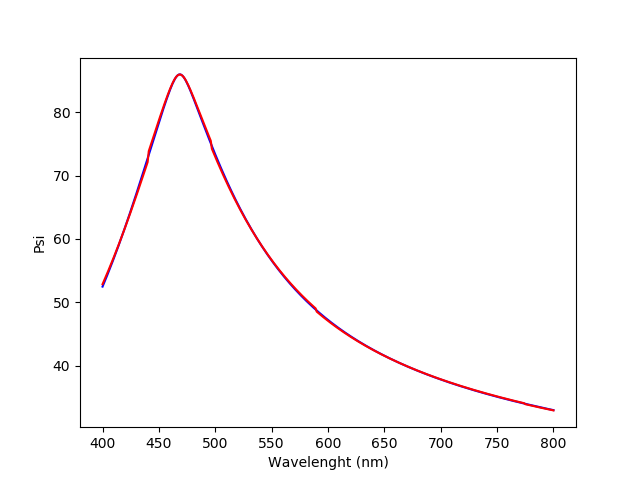
\includegraphics[width=.9\linewidth]{psi.png}
\end{center}

\begin{minted}[]{python}
fig = plt.figure()
plt.plot(csv[:,0],csv[:,2], 'b')
plt.plot(csv[:,0],delta_L, 'r')
plt.ylabel("Delta")
plt.xlabel("Wavelenght (nm)")
plt.savefig("delta.png")
"delta.png"
\end{minted}

\begin{center}
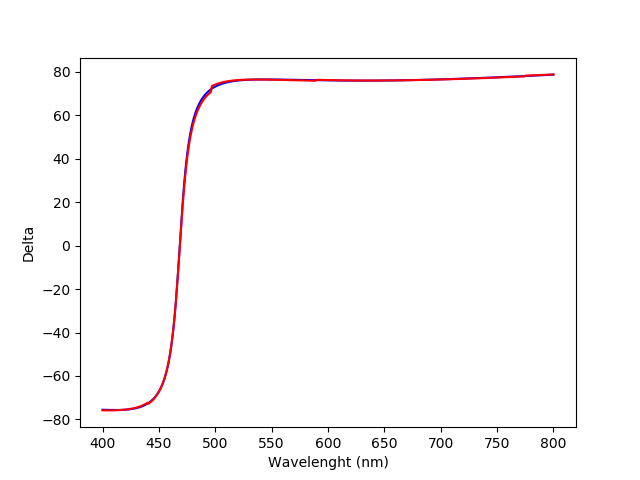
\includegraphics[width=.9\linewidth]{delta.png}
\end{center}


\subsection{Plot refractive index of substrate n\(_{\text{S}}\):}
\label{sec:org3cdb376}

Real part n in blue, imaginary part k in red

\begin{minted}[]{python}
fig = plt.figure()
plt.plot(csv[:,0], csv[:,3], 'b')
plt.plot(csv[:,0], csv[:,4], 'r')
plt.xlabel("wavelength")
plt.ylabel("refractive index of substrate")
plt.savefig("ns.png")
"ns.png"
\end{minted}

\begin{center}
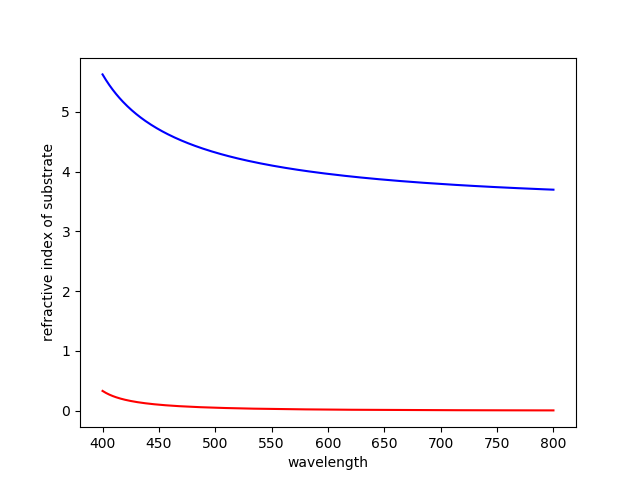
\includegraphics[width=.9\linewidth]{ns.png}
\end{center}
\subsection{Plot real and imaginary part of the created n\(_{\text{L}}\) matrix:}
\label{sec:org2936250}

Real part is blue, imaginary is red.

\begin{minted}[]{python}
fig = plt.figure()
plt.plot(np.real(n_L[:10000]), c='b')
plt.plot(np.imag(n_L[:10000]), c="r")
plt.savefig('n_L.png')
'./n_L.png'
\end{minted}

\begin{center}
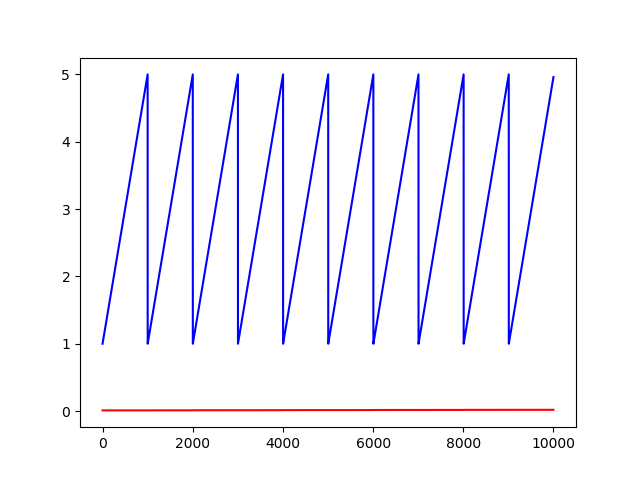
\includegraphics[width=.9\linewidth]{./n_L.png}
\end{center}

\subsection{Plot of the difference between \(\rho_{\text{L}}\) and the given \(\rho\) and determined minimum:}
\label{sec:org8c54f34}

The difference is shown in blue, the red lines show the minimum.

\begin{minted}[]{python}
fig = plt.figure()
plt.axvline(idx, c='r')
plt.axhline(minimum, c='r')
plt.plot(diff)
plt.xlabel("index")
plt.ylabel("difference of rhos")
plt.savefig('diff.png')
"./diff.png"
\end{minted}

\begin{center}
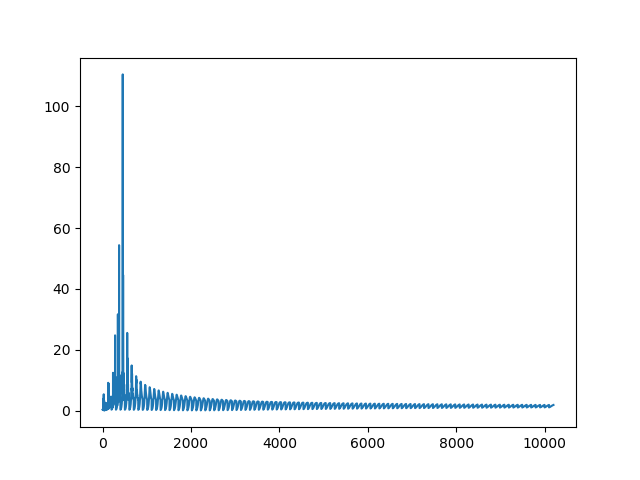
\includegraphics[width=.9\linewidth]{./diff.png}
\end{center}

\subsection{Plot refractive angle phi\(_{\text{L}}\) and n\(_{\text{L}}\):}
\label{sec:org0fab06d}

n\(_{\text{L}}\) is shown in green, real part of phi\(_{\text{L}}\) in blue, imaginary in red. 
A relation between these should be visible.

\begin{minted}[]{python}
fig = plt.figure()
plt.plot(np.real(snell(phi_i, n_air, n_L)[:3000]), 'b')
plt.plot(np.imag(snell(phi_i, n_air, n_L)[:3000]), 'r')
plt.plot(np.real(n_L)[:3000], c='g')
plt.savefig('phi_L.png')
"phi_L.png"
\end{minted}

\begin{center}
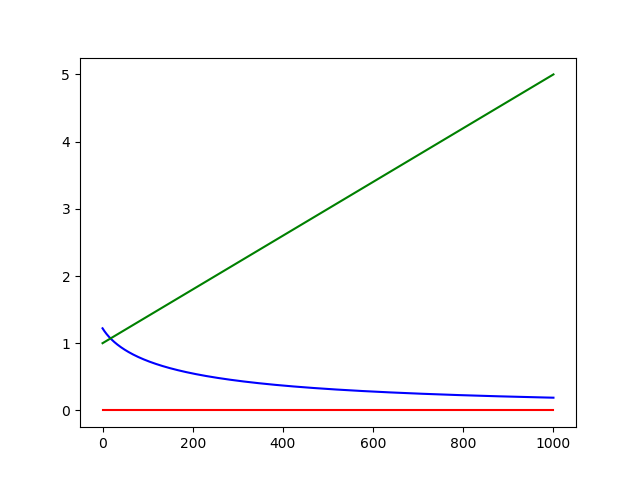
\includegraphics[width=.9\linewidth]{phi_L.png}
\end{center}


\subsection{Plot \(\rho_{\text{given}}\) - \(\rho_{\text{L}}\)}
\label{sec:org853a9da}

Red line shows the found refractive index at the minimum 

\begin{minted}[]{python}
fig = plt.figure()
rho_grid = calc_diff(n_L, rho_giv)
# plt.imshow(rho_grid,origin='lower',extent=(n.min(),n.max(),k.min(),k.max()),
           # aspect = (n.max()-n.min())/(k.max()-k.min()))
# plt.colorbar()
plt.axvline(n_L[idx], c='r')
plt.xlabel('refractive index')
plt.ylabel('abs(rho_given - rho-l)')
plt.axvline(n_array, color="r")
plt.plot(n_L, rho_grid)
# plt.show()
plt.savefig('minimumplot.png') 
"minimumplot.png"
\end{minted}

\begin{center}
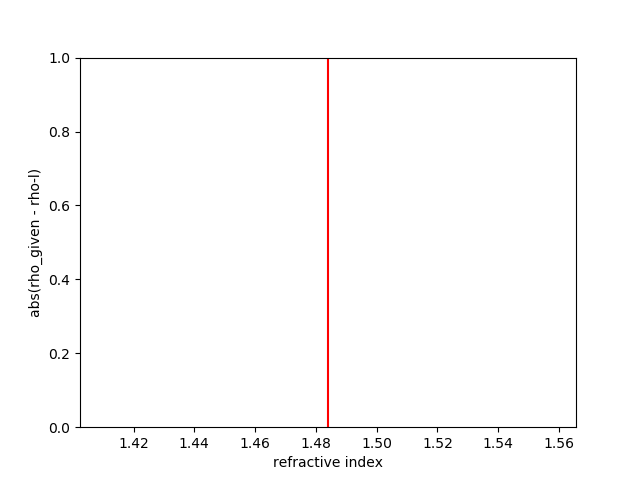
\includegraphics[width=.9\linewidth]{minimumplot.png}
\end{center}

\subsection{Plot n}
\label{sec:orgd80064e}

\begin{minted}[]{python}
fig = plt.figure()
plt.xlabel("wavelenght")
plt.ylabel("refractive index")
plt.plot(csv[:,0], n_array, 'b')
plt.savefig('index.png') 
"index.png"
\end{minted}

\begin{center}
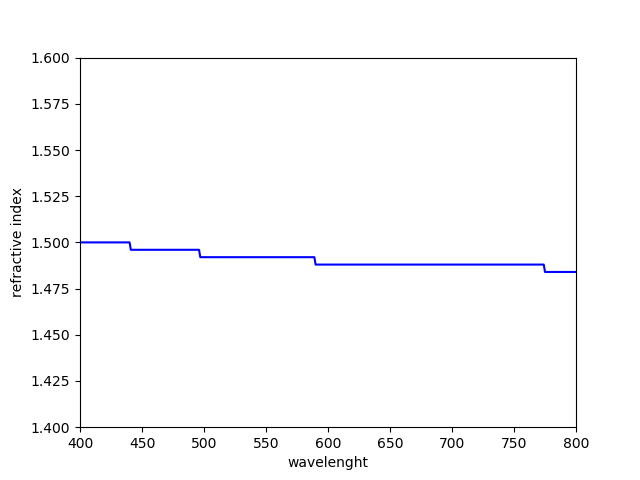
\includegraphics[width=.9\linewidth]{index.png}
\end{center}
\section{Testing:}
\label{sec:org0cbf928}

Testing with constant n\(_{\text{L}}\), phi\(_{\text{i}}\) at i=0
\begin{minted}[]{python}
[("n_L[0]",n_L[0]),("phi_i",phi_i)]
\end{minted}

\subsection{snell():}
\label{sec:org22b0900}

\begin{minted}[]{python}
phi_Ltest = snell(phi_i, n_air, n_L[0])
phi_Ltest
\end{minted}
should be: (1.220429-0.02737074 i)

\begin{minted}[]{python}
("n_S",n_S)
\end{minted}

\begin{minted}[]{python}
phi_Stest = snell(1.220429-0.0273775j,n_L[0],n_S)
phi_Stest
\end{minted}

\begin{center}
\begin{tabular}{l}
0.25693777375213495-0.0029123892267902147j\\
\end{tabular}
\end{center}
should be: (0.151671-0.175494i)



\subsection{fresnel():}
\label{sec:org5b06459}

rs\(_{\text{al}}\), rp\(_{\text{al}}\) = fresnel(n\(_{\text{air}}\), phi\(_{\text{i}}\), n\(_{\text{L}}\), phi\(_{\text{L}}\))

rs\(_{\text{ls}}\), rp\(_{\text{ls}}\) = fresnel(n\(_{\text{L}}\), phi\(_{\text{L}}\), n\(_{\text{S}}\), phi\(_{\text{S}}\))

\begin{minted}[]{python}
rs_altest, rp_altest = fresnel(n_air, phi_i, n_L[0], phi_Ltest)
rs_altest
\end{minted}

\begin{verbatim}
0.0
\end{verbatim}
should be: (-0.003398-0.04239i)
\begin{minted}[]{python}
rp_altest
\end{minted}

\begin{verbatim}
0.0
\end{verbatim}
should be: 

\begin{minted}[]{python}
rs_lstest, rp_lstest = fresnel(n_L[0], phi_Ltest, n_S, phi_Stest)
rs_lstest
\end{minted}

\begin{center}
\begin{tabular}{l}
-0.8254138705368641-0.00029432103501708976j\\
\end{tabular}
\end{center}

\begin{minted}[]{python}
rp_lstest
\end{minted}

\begin{center}
\begin{tabular}{l}
0.13326188486753962+0.0001555019055111361j\\
\end{tabular}
\end{center}

\subsection{calc\(_{\text{rho}}\)():}
\label{sec:orgb7a6c55}

rho\(_{\text{L}}\) = calc\(_{\text{rho}}\)(rs\(_{\text{al}}\), rp\(_{\text{al}}\), rs\(_{\text{ls}}\), rp\(_{\text{ls}}\), d\(_{\text{L}}\), n\(_{\text{L}}\), lambda\(_{\text{vac}}\))
 Just copied this from above with beta returned 
\begin{minted}[]{python}
def calc_rhotest(rs_al, rp_al, rs_ls, rp_ls, d, n, phi, lambda_vac):
    beta = 2 * np.pi * d * n * np.cos(phi) / lambda_vac
    rp_L = (rp_al + rp_ls * np.exp(-2*1j*beta)) / (1 + rp_al * rp_ls * np.exp(-2 * 1j * beta))
    rs_L = (rs_al + rs_ls * np.exp(-2*1j*beta)) / (1 + rs_al * rs_ls * np.exp(-2 * 1j * beta))
    rho_L = rp_L / rs_L
    return rho_L, beta
\end{minted}

\begin{minted}[]{python}
rhotest, betatest = calc_rhotest(rs_altest, rp_altest, rs_lstest, rp_lstest, 300, n_L[0], phi_Ltest, lambda_vac)
betatest
\end{minted}

\begin{verbatim}
0.805865977238737
\end{verbatim}
should be: 2.1558487+0.18312240i

\begin{minted}[]{python}
rhotest 
\end{minted}

\begin{center}
\begin{tabular}{l}
-0.16144861157373563-0.00013082428937188695j\\
\end{tabular}
\end{center}



\bibliography{forschungspraktikum}
\end{document}